% fig17-intervention-taxonomy.tex
% Intervention outcome taxonomy: replicate / reroute / collapse
\documentclass[tikz,border=18pt]{standalone}
% common-styles.tex
% Shared TikZ styles for wonton-proof paper figures

\usepackage{silence}
\WarningFilter{latex}{Missing character} 
\tracinglostchars=0 % Suppress engine-level "Missing character" warnings

\usepackage{fontspec}
\usepackage{unicode-math}

% Use filenames for reliability with Tectonic
\setmainfont{LibertinusSerif-Regular.otf}[
    BoldFont=LibertinusSerif-Bold.otf,
    ItalicFont=LibertinusSerif-Italic.otf,
    BoldItalicFont=LibertinusSerif-BoldItalic.otf
]
\setsansfont{LibertinusSans-Regular.otf}[
    BoldFont=LibertinusSans-Bold.otf,
    ItalicFont=LibertinusSans-Italic.otf
]
\setmonofont{LibertinusMono-Regular.otf}

% Try a more standard math font if LibertinusMath is causing nullfont issues
\setmathfont{LibertinusMath-Regular.otf}
% \setmathfont{latinmodern-math.otf}[range=digits] 

\usepackage{amsmath}
\usepackage{tikz}
\usepackage{forest}

\usetikzlibrary{
    arrows.meta,
    calc,
    decorations.pathreplacing,
    fit,
    positioning,
    shapes.geometric,
    shapes.misc,
    backgrounds,
    shadows.blur,
    fadings
}

% Color palette (muted, print-friendly)
\definecolor{ink}{RGB}{45,45,52}
\definecolor{muted}{RGB}{115,115,125}
\definecolor{highlight}{RGB}{198,120,44}
\definecolor{accentblue}{RGB}{86,130,178}
\definecolor{accentgreen}{RGB}{84,156,132}
\definecolor{blocked}{RGB}{140,75,75}
\definecolor{goalnode}{RGB}{255,255,255}
\definecolor{terminal}{RGB}{238,239,244}
\definecolor{deadnode}{RGB}{248,245,245}
\definecolor{flowbox}{RGB}{250,250,252}
\definecolor{basin1}{RGB}{224,234,248}
\definecolor{basin2}{RGB}{246,232,221}
\definecolor{basin3}{RGB}{228,242,234}
\definecolor{heatbase}{RGB}{86,130,178}

\tikzset{
    line cap=round,
    line join=round,
    pop/.style={
        blur shadow={shadow blur steps=5, shadow blur extra rounding=1.3pt}
    },
    base node/.style={
        rounded rectangle,
        draw=ink,
        line width=0.6pt,
        fill=goalnode,
        text=ink,
        minimum width=2.2cm,
        minimum height=0.7cm,
        align=center,
        pop
    },
    goal/.style={base node, fill=goalnode},
    terminal/.style={base node, fill=terminal, line width=0.9pt},
    dead/.style={base node, fill=deadnode, dashed},
    flowbox/.style={
        rectangle,
        draw=muted,
        rounded corners=3pt,
        fill=flowbox,
        minimum width=1.8cm,
        minimum height=0.6cm,
        align=center,
        font=\normalfont\small,
        text=ink,
        pop
    },
    decision/.style={
        diamond,
        draw=muted,
        fill=flowbox,
        aspect=2.4,
        font=\normalfont\small,
        inner sep=1pt,
        text=ink
    },
    protocolbox/.style={
        rectangle,
        draw=muted,
        rounded corners=4pt,
        fill=flowbox,
        minimum width=2cm,
        minimum height=0.8cm,
        font=\normalfont\small,
        align=center,
        text=ink
    },
    tactic/.style={
        ->,
        >=Stealth,
        draw=muted,
        line width=0.75pt
    },
    tacticlight/.style={
        ->,
        >=Stealth,
        draw=muted!45,
        dashed,
        line width=0.6pt
    },
    backprop/.style={
        ->,
        >=Stealth,
        draw=muted!70,
        dashed,
        line width=0.6pt
    },
    selected/.style={
        tactic,
        draw=highlight,
        line width=1.4pt
    },
    divergetactic/.style={
        tactic,
        draw=highlight,
        line width=1.4pt
    },
    divergenode/.style={
        base node,
        draw=highlight,
        line width=1.0pt
    },
    divergeblock/.style={
        blockedtactic,
        line width=1.2pt
    },
    blockedtactic/.style={
        tactic,
        draw=blocked,
        densely dashed
    },
    flowarrow/.style={
        ->,
        >=Stealth,
        draw=muted,
        line width=0.75pt
    },
    crosslink/.style={
        -,
        draw=muted!70,
        dotted,
        line width=0.6pt
    },
    annot/.style={
        font=\normalfont\footnotesize,
        text=muted
    },
    visit/.style={
        annot,
        font=\normalfont\scriptsize
    },
    annotbg/.style={
        annot,
        fill=white,
        inner sep=1.5pt
    },
    tacticlabel/.style={
        annot,
        font=\ttfamily\footnotesize,
        text=muted
    },
    formula/.style={
        font=\normalfont\footnotesize,
        draw=muted,
        rounded corners=2pt,
        fill=white,
        inner sep=3pt
    },
    paneltitle/.style={
        font=\normalfont\bfseries,
        text=ink
    },
    trajectory/.style={
        ->,
        draw=muted!70,
        line width=0.6pt
    }
}


\begin{document}
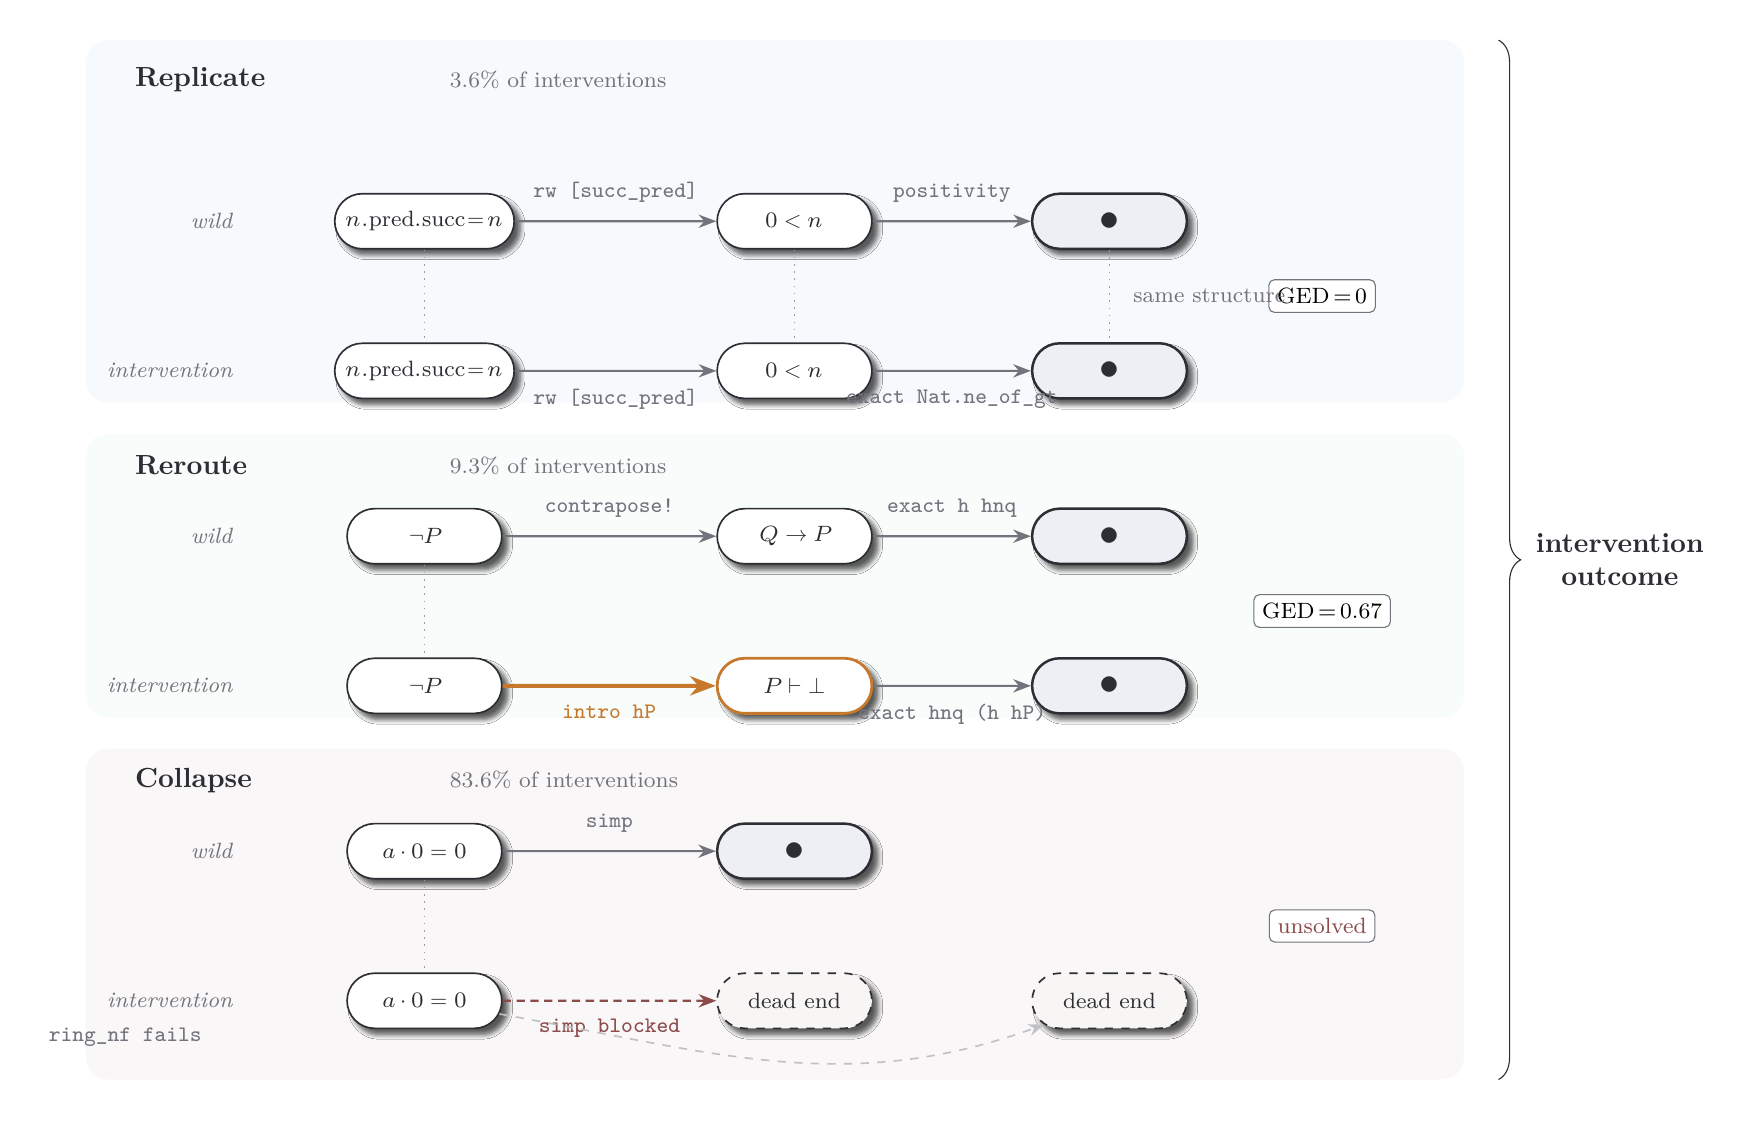
\begin{tikzpicture}[
    every node/.style={font=\small},
    show background rectangle,
    background rectangle/.style={fill=white},
    treenode/.style={base node, minimum width=2.0cm, minimum height=0.65cm}
]

\def\rowsep{1.9}

% Lane backgrounds
\path[fill=basin1!25, rounded corners=8pt]
    (-0.5, 7.0) rectangle (17.0, 11.6);
\path[fill=basin3!25, rounded corners=8pt]
    (-0.5, 3.0) rectangle (17.0, 6.6);
\path[fill=deadnode!80, rounded corners=8pt]
    (-0.5, -1.6) rectangle (17.0, 2.6);

% === REPLICATE (top lane) ===
% nat_succ_pred / block positivity (GED = 0)
\begin{scope}[shift={(0, 7.4)}]
    \node[paneltitle, anchor=west] at (0, 3.7) {Replicate};
    \node[annot, anchor=west] at (4.0, 3.7) {3.6\% of interventions};

    % Wild-type path
    \node[annot, anchor=east] at (1.5, \rowsep) {\textit{wild}};
    \node[treenode, goal] (rw0) at (3.8, \rowsep) {\footnotesize$n.\text{pred}.\text{succ}\!=\!n$};
    \node[treenode, goal] (rw1) at (8.5, \rowsep) {\footnotesize$0 < n$};
    \node[treenode, terminal] (rwt) at (12.5, \rowsep) {{\Large$\bullet$}};
    \draw[tactic] (rw0) -- (rw1)
        node[midway, above=3pt, tacticlabel] {\texttt{rw [succ\_pred]}};
    \draw[tactic] (rw1) -- (rwt)
        node[midway, above=3pt, tacticlabel] {\texttt{positivity}};

    % Intervention path
    \node[annot, anchor=east] at (1.5, 0) {\textit{intervention}};
    \node[treenode, goal] (ri0) at (3.8, 0) {\footnotesize$n.\text{pred}.\text{succ}\!=\!n$};
    \node[treenode, goal] (ri1) at (8.5, 0) {\footnotesize$0 < n$};
    \node[treenode, terminal] (rit) at (12.5, 0) {{\Large$\bullet$}};
    \draw[tactic] (ri0) -- (ri1)
        node[midway, below=3pt, tacticlabel] {\texttt{rw [succ\_pred]}};
    \draw[tactic] (ri1) -- (rit)
        node[midway, below=3pt, tacticlabel] {\texttt{exact Nat.ne\_of\_gt}};

    % GED badge
    \node[formula] at (15.2, \rowsep/2) {GED\,=\,0};

    % Cross links
    \draw[crosslink] (rw0.south) -- (ri0.north);
    \draw[crosslink] (rw1.south) -- (ri1.north);
    \draw[crosslink] (rwt.south) -- (rit.north)
        node[midway, right=5pt, annot] {\footnotesize same structure};
\end{scope}

% === REROUTE (middle lane) ===
% contrapositive / block contrapose! (GED = 0.67)
\begin{scope}[shift={(0, 3.4)}]
    \node[paneltitle, anchor=west] at (0, 2.8) {Reroute};
    \node[annot, anchor=west] at (4.0, 2.8) {9.3\% of interventions};

    % Wild-type path
    \node[annot, anchor=east] at (1.5, \rowsep) {\textit{wild}};
    \node[treenode, goal] (mw0) at (3.8, \rowsep) {\footnotesize$\neg P$};
    \node[treenode, goal] (mw1) at (8.5, \rowsep) {\footnotesize$Q \to P$};
    \node[treenode, terminal] (mwt) at (12.5, \rowsep) {{\Large$\bullet$}};
    \draw[tactic] (mw0) -- (mw1)
        node[midway, above=3pt, tacticlabel] {\texttt{contrapose!}};
    \draw[tactic] (mw1) -- (mwt)
        node[midway, above=3pt, tacticlabel] {\texttt{exact h hnq}};

    % Intervention path (different structure highlighted)
    \node[annot, anchor=east] at (1.5, 0) {\textit{intervention}};
    \node[treenode, goal] (mi0) at (3.8, 0) {\footnotesize$\neg P$};
    \node[treenode, divergenode] (mi1) at (8.5, 0) {\footnotesize$P \vdash \bot$};
    \node[treenode, terminal] (mit) at (12.5, 0) {{\Large$\bullet$}};
    \draw[divergetactic] (mi0) -- (mi1)
        node[midway, below=3pt, tacticlabel, text=highlight] {\texttt{intro hP}};
    \draw[tactic] (mi1) -- (mit)
        node[midway, below=3pt, tacticlabel] {\texttt{exact hnq (h hP)}};

    % GED badge
    \node[formula] at (15.2, \rowsep/2) {GED\,=\,0.67};

    % Cross link (roots only -- different structure so no terminal link)
    \draw[crosslink] (mw0.south) -- (mi0.north);
\end{scope}

% === COLLAPSE (bottom lane) ===
% block simp (573/573 fail)
\begin{scope}[shift={(0, -0.6)}]
    \node[paneltitle, anchor=west] at (0, 2.8) {Collapse};
    \node[annot, anchor=west] at (4.0, 2.8) {83.6\% of interventions};

    % Wild-type path (simp solves directly)
    \node[annot, anchor=east] at (1.5, \rowsep) {\textit{wild}};
    \node[treenode, goal] (cw0) at (3.8, \rowsep) {\footnotesize$a \cdot 0 = 0$};
    \node[treenode, terminal] (cwt) at (8.5, \rowsep) {{\Large$\bullet$}};
    \draw[tactic] (cw0) -- (cwt)
        node[midway, above=3pt, tacticlabel] {\texttt{simp}};

    % Intervention path (blocked, nothing else works)
    \node[annot, anchor=east] at (1.5, 0) {\textit{intervention}};
    \node[treenode, goal] (ci0) at (3.8, 0) {\footnotesize$a \cdot 0 = 0$};
    \node[treenode, dead] (ci1) at (8.5, 0) {\footnotesize dead end};
    \node[treenode, dead] (ci2) at (12.5, 0) {\footnotesize dead end};
    \draw[blockedtactic] (ci0) -- (ci1)
        node[midway, below=3pt, tacticlabel, text=blocked] {\texttt{simp} blocked};
    \draw[tacticlight] (ci0) to[out=-10, in=200] (ci2)
        node[pos=0.5, below=6pt, tacticlabel] {\texttt{ring\_nf} fails};

    % Badge
    \node[formula, text=blocked] at (15.2, \rowsep/2) {unsolved};

    % Cross link
    \draw[crosslink] (cw0.south) -- (ci0.north);
\end{scope}

% Right-side brace
\draw[decorate, decoration={brace, amplitude=8pt, mirror, raise=4pt}, ink]
    (17.3, -1.6) -- (17.3, 11.6)
    node[midway, right=14pt, paneltitle, align=center] {intervention\\outcome};

\end{tikzpicture}
\end{document}
